\section*{presentazione}

\begin{itemize}
  \item presentazione
  \item ringraziamenti e scuse presenza
  \item LEAP vs Conservatorio
  \item ricerca indipendente, LEAP, LAZZARO
  \item \emph{perché siamo qui?}: esperienza musicale.
\end{itemize}

%\clearpage

\section{punctum}

\begin{figure}[htbp]
\begin{center}
\frame{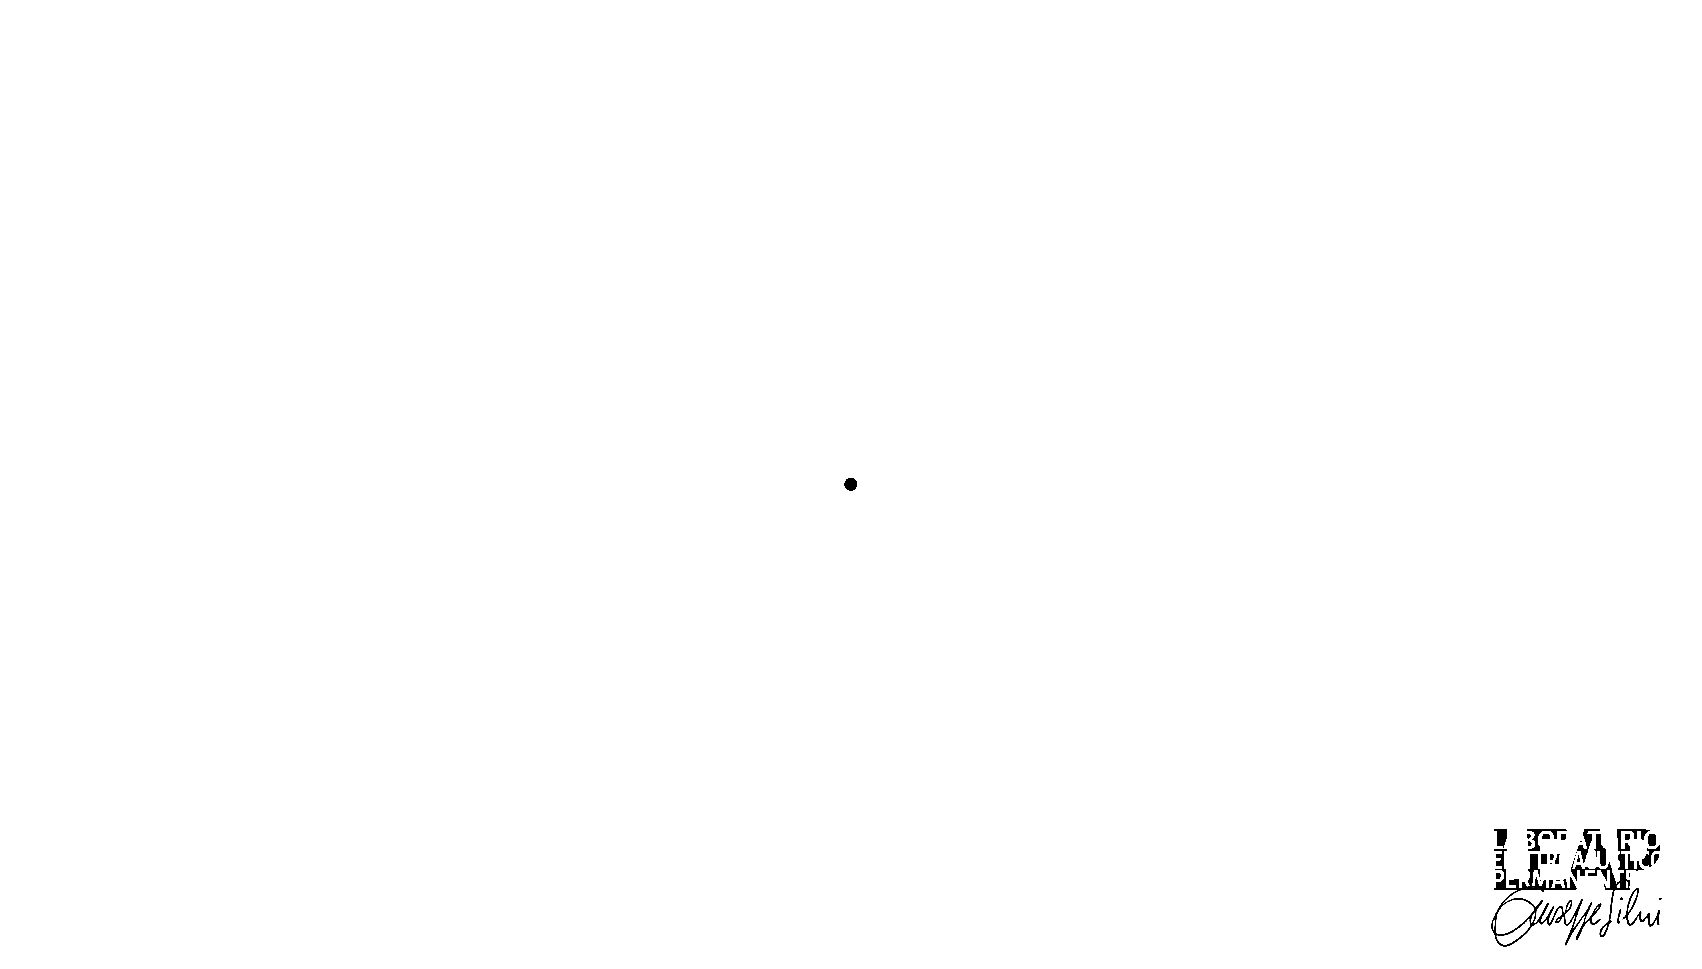
\includegraphics[width=0.9\textwidth]{presentazione/001-cua-presentazione-gatm.pdf}}
\caption{punctum}
\label{slide1}
\end{center}
\end{figure}

\begin{quote}
  Tutto quello di cui Euclide parla, non esiste. [\ldots] L'immaginazione che Euclide [\ldots] richiede a chi legge i suoi \emph{Elementi} è più grande di quella necessaria a seguire le storie degli dèi e degli eroi. [\ldots] Il punto, come Euclide lo definisce, è ciò che non ha parti. Non si può attraccare al punto, afferrare il punto, circumnavigare il punto e nemmeno si potrebbe mettere un punto. [\ldots] Una immaginazione che non trasforma ma crea. Che non è metamorfosi, ma invenzione. [\ldots] D'altronde i punti, soli o allineati stretti a formare rette o piani, sono gli elementi dell'unica grammatica che, oltre a descrivere e comunicare il mondo, ha permesso di costruire e gestire dispositivi che ci hanno mandato oltre le stelle fisse, e più in là. \cite{valerio16}
\end{quote}

Strappando parole di Chiara Valerio dalle prime pagine di \emph{Storia umana della matematica}, introduco il punto come entità geometrica \emph{senza forma e senza dimensione} - solo posizione, senza estensione - come simbolo centrale e imprescindibile di questo lavoro. Il \emph{punctum} è, oltre le sue quantità geometriche, l'astrazione di un foro, un buco, di una trafittura, l'astratto di una posizione, di un momento, la questione specifica di un luogo. Quando diciamo «questo è il punto» o «a che punto siamo?» conserviamo l'idea di qualcosa di preciso, determinato, localizzato, come la traccia di un oggetto appuntito sulla materia, con la precisione della localizzazione. Con questa polisemica precisione astratta, con le invenzioni euclidee, richiamo, geolocalizzo, la nozione bergsoniana di virtualità pura\footnote{%
  Virtuale deriva dal latino \emph{virtualis}, da \emph{virtus} (“forza, potenza, capacità”), che a sua volta viene da \emph{vir} (“uomo, forza virile”). Il virtuale è dunque ciò che possiede la \emph{virtus}, la potenza di essere, anche se non è attualmente manifesto. Per Bergson, \textbf{il virtuale non si oppone al reale, ma all'attuale}: il virtuale è pienamente reale, esiste con una modalità d'essere propria, ma non è presente, non è attualizzato nella percezione o nella coscienza. Il possibile, è ciò che non esiste ancora e potrebbe venire all'esistenza – il virtuale già esiste, ma in modo diverso dall'attuale. La memoria pura bergsoniana è la forma paradigmatica della virtualità. Il passato non scompare, ma persiste integralmente come virtualità: tutto ciò che abbiamo vissuto continua a esistere, non come traccia cerebrale o rappresentazione, ma come passato puro che coesiste col presente. Questa totalità mnemonica virtuale non è immediatamente accessibile alla coscienza – sarebbe paralizzante – ma permane come sfondo ontologico. Quando ricordiamo, non riproduciamo un'immagine archiviata nel cervello, ma compiamo un movimento di attualizzazione: ci contraiamo verso un livello specifico di questa memoria virtuale, e ne estraiamo ricordi-immagini che si incarnano nella percezione presente. Il ricordo non era “da qualche parte” in attesa: era virtuale, e diventa attuale attraverso lo sforzo di memoria. Nel celebre schema del cono, Bergson rappresenta il passato come una totalità virtuale (la base del cono) che si contrae progressivamente verso il vertice (il presente, l'azione) - un punto. L'attualizzazione è questo movimento di contrazione, non una selezione tra rappresentazioni discrete, ma una modulazione continua tra diversi piani di virtualità.
}.

Parto quindi da una forma inesistente, dall'idea di, dall'immaginazione, dalla fantasia «che non trasforma ma crea. Che non è metamorfosi, ma invenzione» per ri-portare al centro del dialogo sulla musica un \emph{antico punto}, la memoria, verso l'esplorazione dell'esperienza musicale.

\section{memoria}

\begin{figure}[h]
\begin{center}
\frame{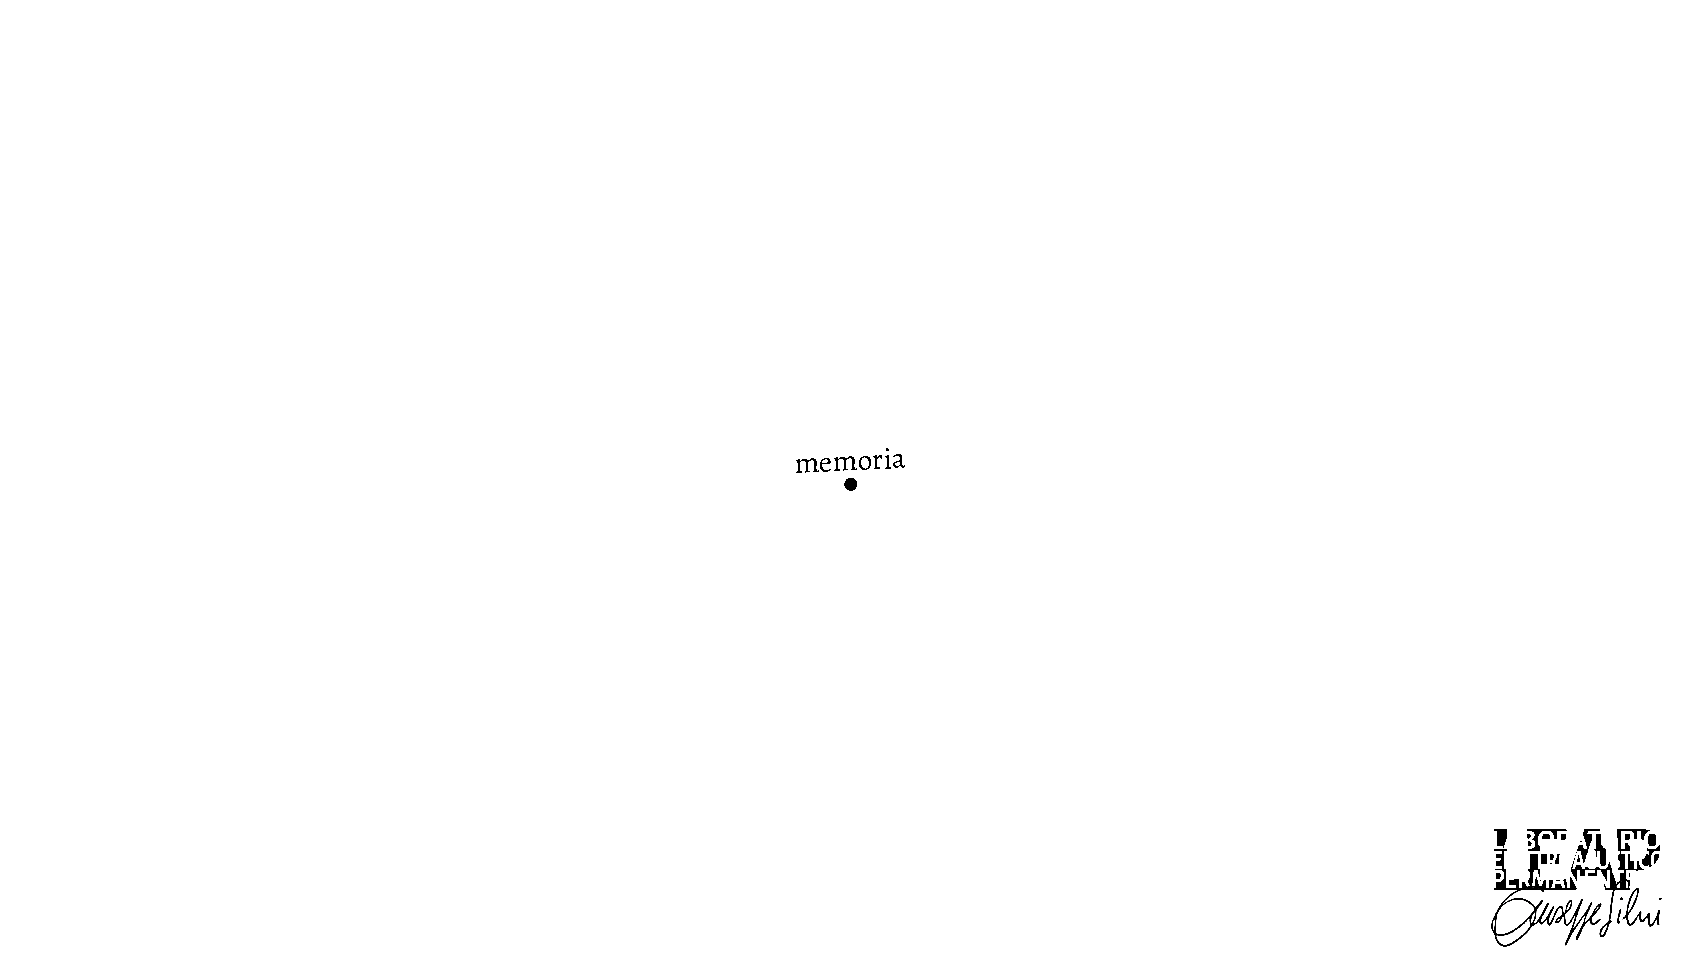
\includegraphics[width=0.9\textwidth]{presentazione/002-cua-presentazione-gatm.pdf}}
\caption{memoria}
\label{slide2}
\end{center}
\end{figure}

Memoria deriva dal latino \emph{memoria}, sostantivo femminile che ha la sua radice nel verbo \emph{memini} (“ricordare”, “essere memore”). Questo verbo appartiene alla famiglia indo-europea {\phonfont *men-}, che indica l'attività mentale del pensare e ricordare. La stessa radice si ritrova in greco antico \textgreek{μνήμη} (\emph{mneme}) e \textgreek{μνῆμα} (\emph{mnema}), da cui derivano termini come “mnemonica” e “amnesia”.

Il suffisso \emph{-ia} forma il sostantivo astratto dalla radice aggettivale \emph{memor} (“memore, che ricorda”), indicando originariamente una facoltà o capacità mentale: la memoria come potenza del ricordare. Tuttavia, già nella tradizione retorica e filosofica antica, la memoria venne concepita anche come \emph{locus et instrumentum} mentale – luogo di deposito e strumento di richiamo. Questa duplicità tra facoltà astratta e topologia operativa attraversa l'intera storia del concetto: dai \emph{loci memoriae} della mnemotecnica ciceroniana fino alle metafore moderne dell'archivio e della traccia.

Questa tensione etimologico-concettuale stratifica un potenziale dinamico che oggi possiamo articolare in una memoria preservante, in una durata sedimentante, per una ritenzione attualizzante\footnote{%
 Il passaggio dalla memoria-archivio alla memoria-processo attraversa la filosofia del Novecento: Bergson in \emph{Matière et mémoire} (1896) distingue tra memoria-abitudine (automatica, corporea) e memoria pura (virtuale), concependo il ricordo non come riproduzione meccanica ma come \emph{actualisation du virtuel} – attualizzazione creativa nel presente. Husserl nelle \emph{Vorlesungen zur Phänomenologie des inneren Zeitbewußtseins} (1905-1910) radicalizza questa temporalità introducendo \emph{Retention} e \emph{Protention}: la coscienza si costituisce trattenendo l'appena-passato e anticipando il subito-futuro, rendendo la memoria struttura trascendentale della temporalità stessa. Merleau-Ponty in \emph{Phénoménologie de la perception} (1945) incarna questa temporalità nel corpo proprio: la memoria diventa sedimentazione corporea, schema motorio, processualità incarnata. Heidegger in \emph{Sein und Zeit} (1927) ontologizza ulteriormente il \emph{Gedächtnis}, non più facoltà psicologica ma modo d'essere del \emph{Dasein}: la memoria come \emph{Wiederholung} (ripresa) che apre il futuro attraverso la riappropriazione autentica del passato. Derrida in \emph{Mal d'archive} (1995) decostruisce la presenza mnemonica: la memoria è \emph{trace} e \emph{différance}, archivio che si produce nell'archiviazione stessa, mai pienamente presente a sé. Ricœur in \emph{La mémoire, l'histoire, l'oubli} (2000) elabora la memoria come \emph{travail} – processo ermeneutico e dialettico tra presenza e assenza, fedeltà e tradimento, che configura l'identità narrativa. Infine, la filosofia processuale porta a compimento questa trasformazione: Whitehead in \emph{Process and Reality} (1929) pensa l'esperienza come \emph{prehension} cumulativa, mentre Deleuze in \emph{Bergsonisme} (1966) radicalizza la virtualità bergsoniana come produzione continua di connessioni, \emph{éternel retour de la différence}, forza creativa che determina il divenire.
}.

In questa prospettiva, \emph{memorare} non significa conservare ma processare - trasformare continuamente il passato nel presente, facendo della memoria non un archivio ma un laboratorio temporale della soggettività.

\section{memoria come luogo}

\begin{figure}[htbp]
\begin{center}
\frame{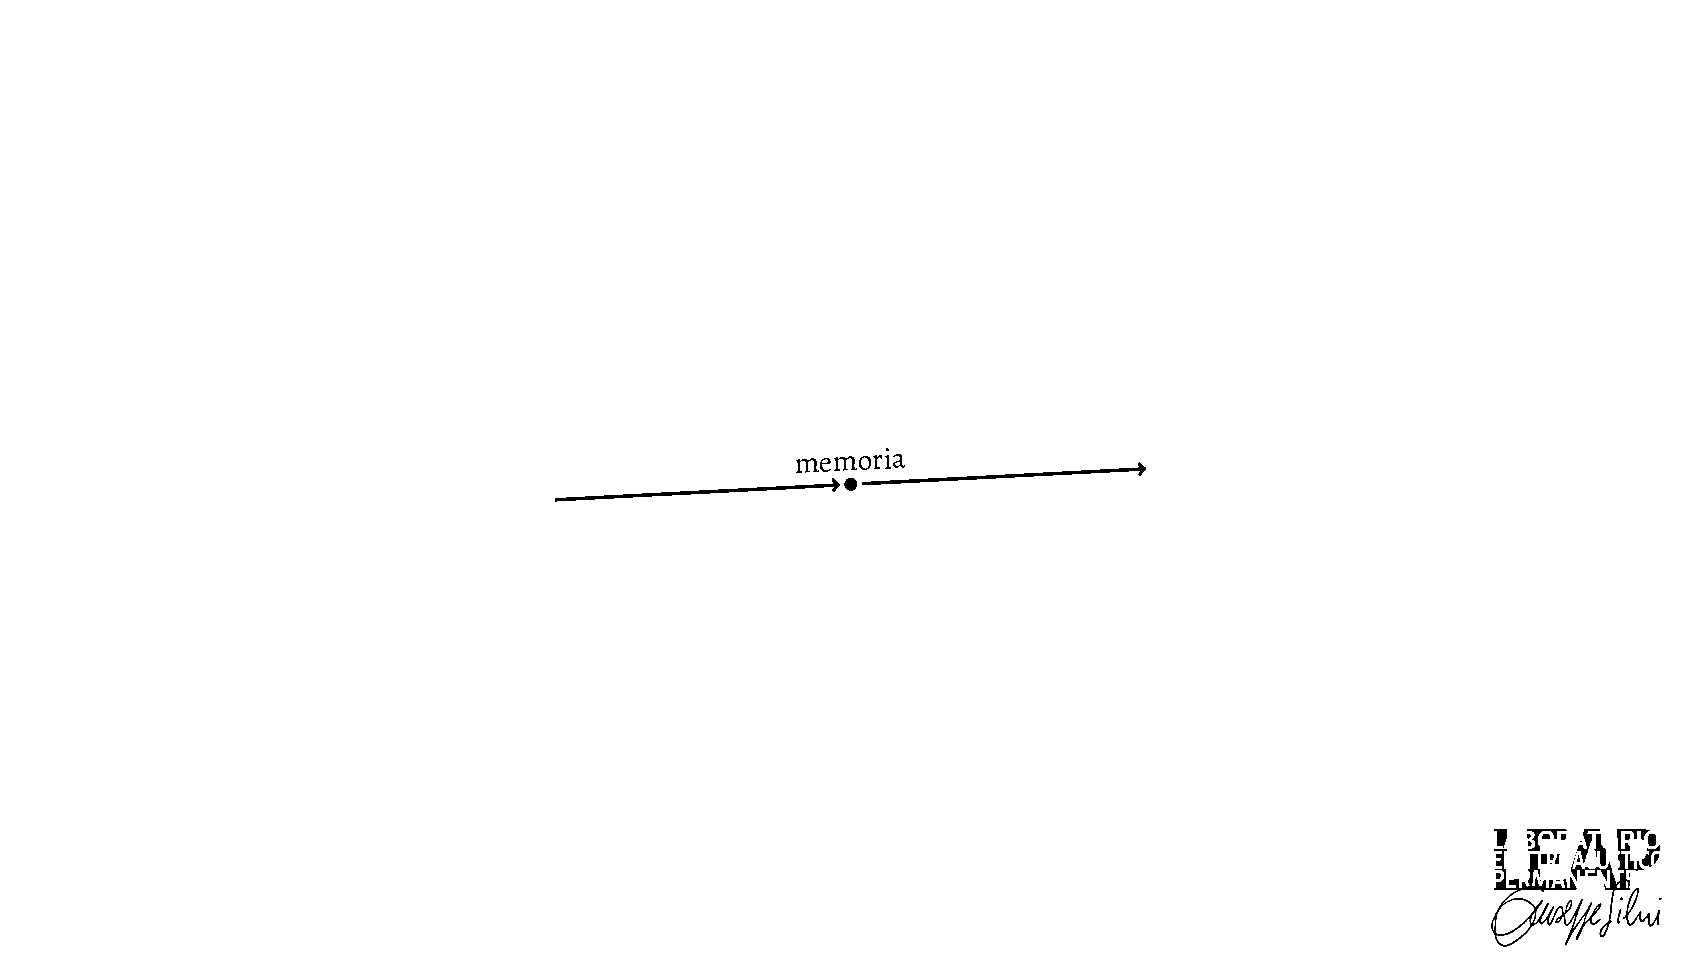
\includegraphics[width=0.9\textwidth]{presentazione/003-cua-presentazione-gatm.pdf}}
\caption{memoria come luogo con almeno un ingresso e un'uscita.}
\label{slide3}
\end{center}
\end{figure}

La memoria come luogo, senza dimensione né forma, deve avere almeno un ingresso e un'uscita. Questa topografizzazione della memoria mi permette di introdurre un verso, una direzione, un'idea di flusso. L'ingresso è deposizione, l'uscita è attualizzazione – tra i due, il laboratorio temporale opera la sua trasformazione.

\section{memoria come passaggio}

\begin{figure}[htbp]
\begin{center}
\frame{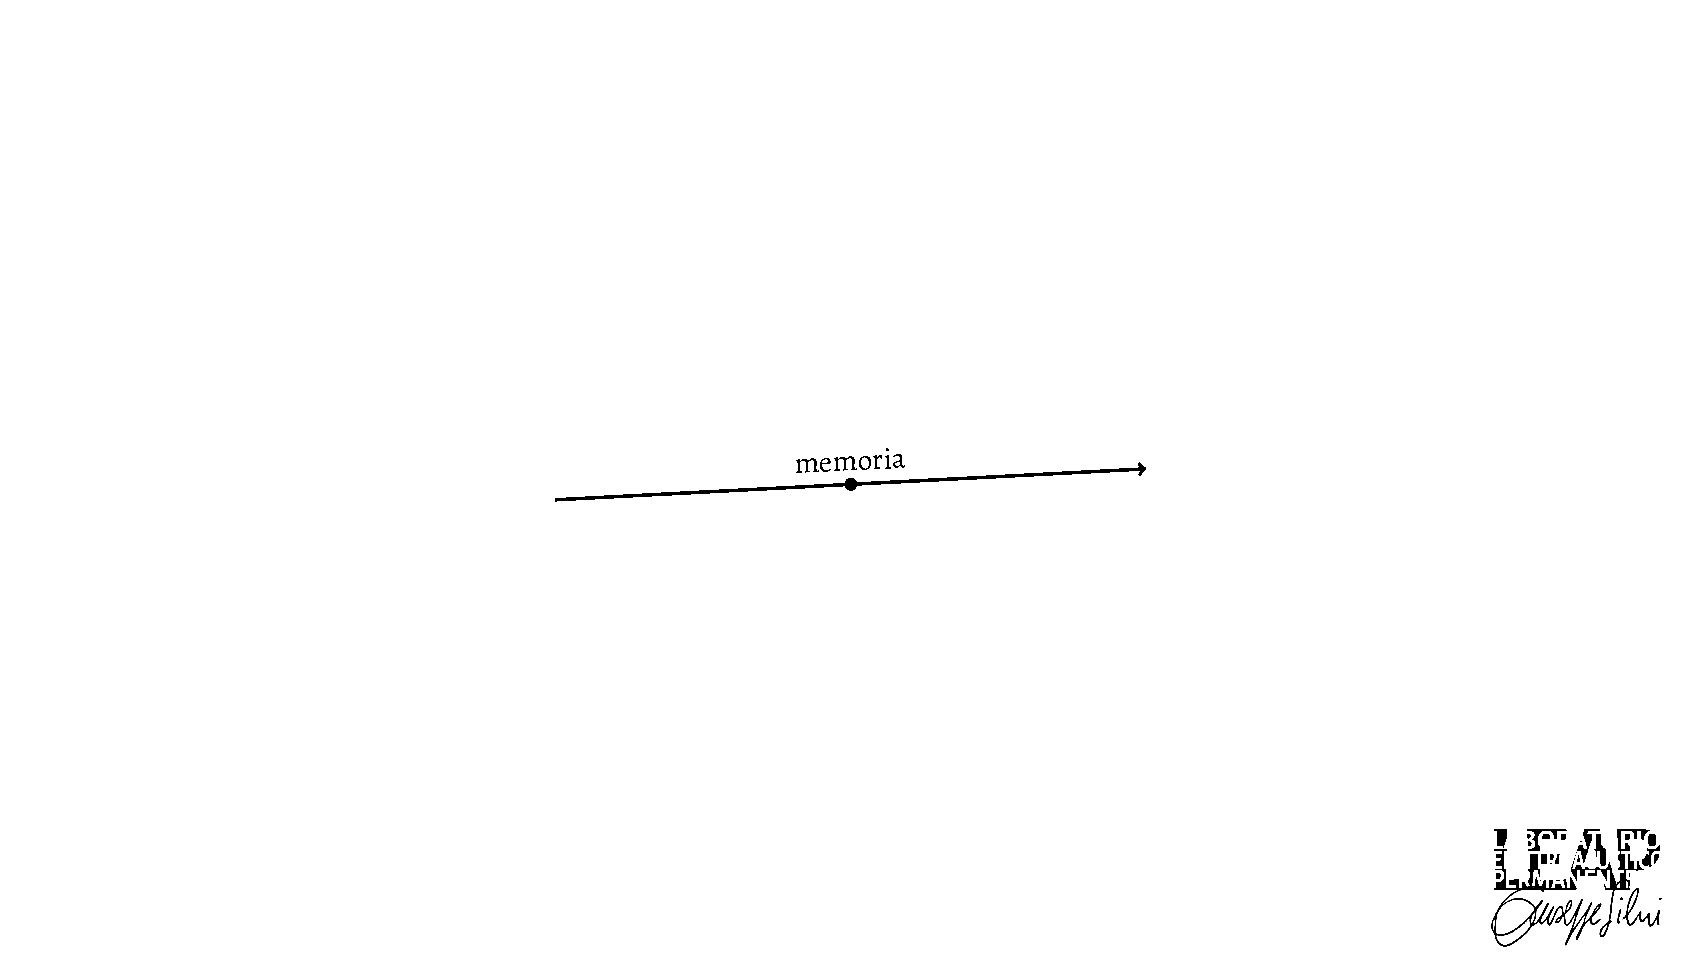
\includegraphics[width=0.9\textwidth]{presentazione/004-cua-presentazione-gatm.pdf}}
\caption{memoria come passaggio, attraversamento.}
\label{slide4}
\end{center}
\end{figure}

Il luogo diviene passaggio, attraversamento. Non più due momenti separati – l'entrare e l'uscire – ma un unico movimento continuo di cui la memoria è il \emph{medium}. Il luogo rimane ma si dissolve nell'attraversamento: la memoria non sta più tra ingresso e uscita, ma è l'attraversamento stesso. Qui si compie la trasformazione da entità a processo, da sostanza a verbo\footnote{%
  L'approccio adottato in questa ricerca muove dalla convinzione che la memoria tecnologica (buffer, RAM, storage) non sia semplice simulazione della memoria umana, ma dispositivo che materializza e rende operativa quella concezione processuale elaborata dalla filosofia novecentesca. I concetti di sedimentazione, ritenzione, traccia diventano così criteri analitici per comprendere le temporalità dei media digitali.
}.

\section{elaborazione del segnale}

\begin{figure}[htbp]
\begin{center}
\frame{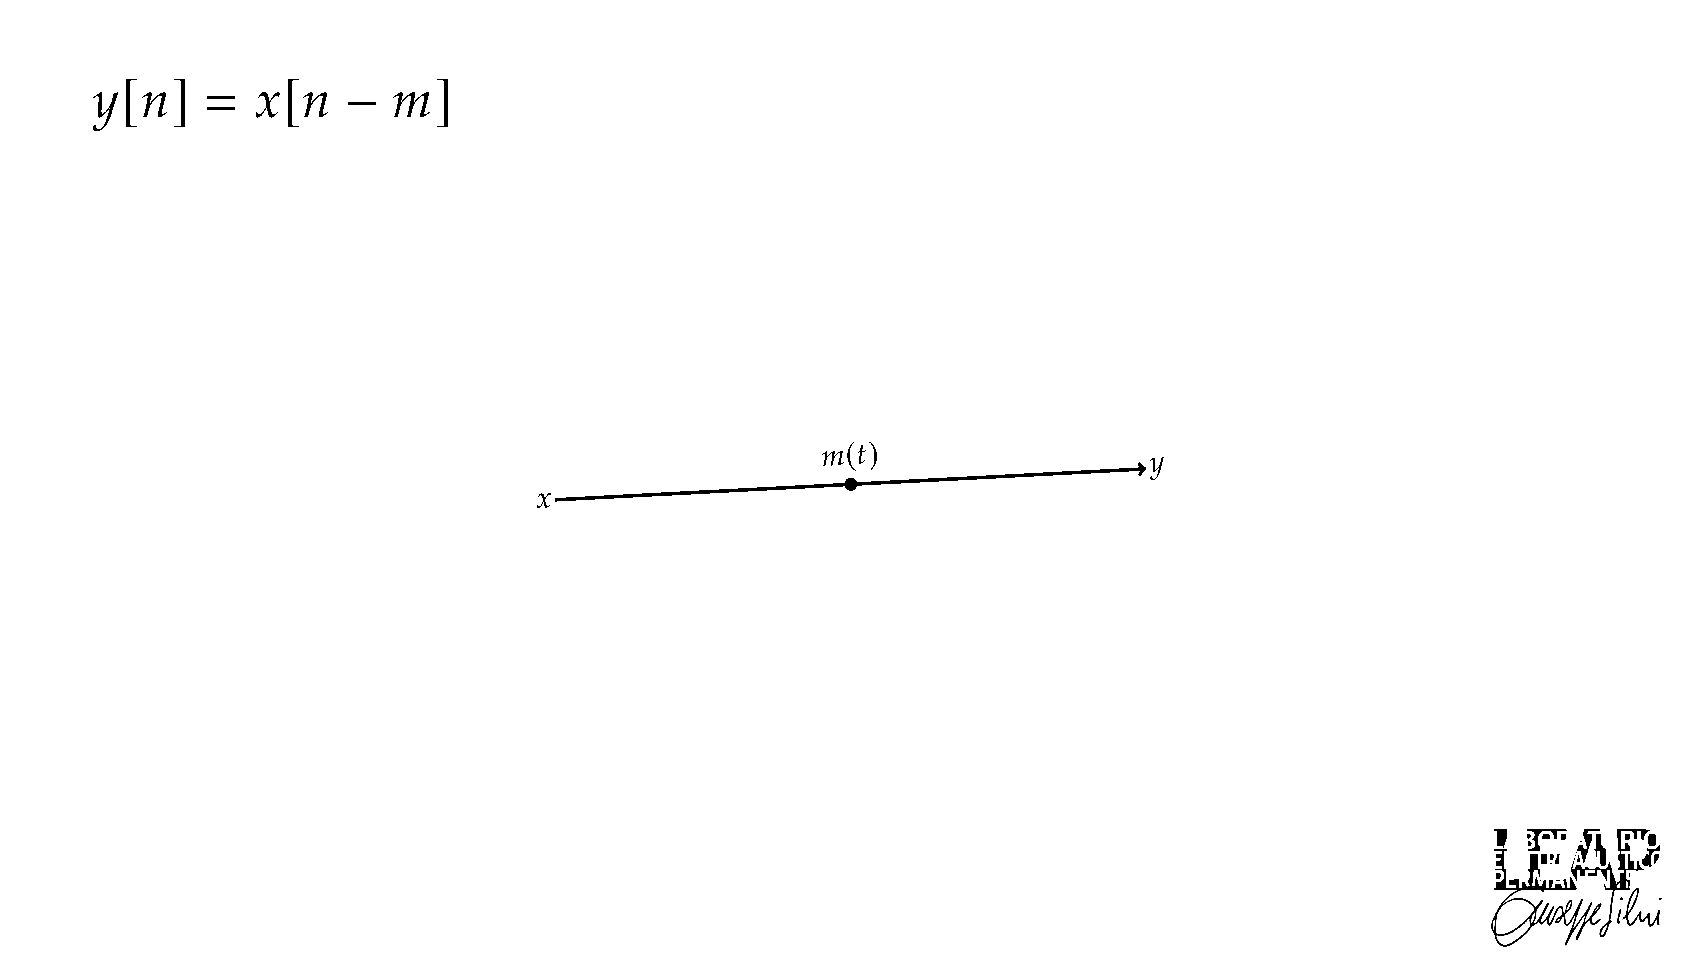
\includegraphics[width=0.9\textwidth]{presentazione/005-cua-presentazione-gatm.pdf}}
\caption{memoria come elaborazione di un segnale in transito.}
\label{slide5}
\end{center}
\end{figure}

Segno deriva dal latino \emph{signum}, che ha la sua radice nella famiglia indoeuropea {\phonfont *sek-} (“tagliare, incidere, separare”). Il segno nasce da un gesto di incisione: tracciare una marca, operare una distinzione, separare questo da quello. È l'atto che estrae una forma dal continuum, che introduce la cesura nel flusso.

Segnale, dal latino medievale \emph{signale} (formato da \emph{signum} + il suffisso \emph{-ale}), aggiunge al segno una dimensione operativa e vettoriale: non più solo traccia statica, ma indicazione dinamica, chiamata all'azione, anticipazione di movimento.

Per Bergson, il segno è l'operazione intellettuale che fissa il movimento del reale, l'impronta negativa della durata\footnote{%
  In \emph{L'évolution créatrice} (1907), Bergson analizza come l'intelligenza operi per spatializzazione e discretizzazione del continuo. Il concetto, il simbolo, il segno sono gli strumenti attraverso cui l'intelletto sostituisce la fluidità del reale con rappresentazioni statiche e manipolabili. Questa operazione è necessaria per l'azione pratica, ma tradisce ontologicamente il movimento della vita: l'intelligenza «envisagée dans ce qui en paraît être la démarche originelle, est la faculté de fabriquer des objets artificiels, en particulier des outils à faire des outils, et d'en varier indéfiniment la fabrication» (L'évolution créatrice, p. 140). Il segno è lo strumento di questa fabbricazione, ciò che permette di trattare il reale come se fosse composto di elementi discreti e ricombinabili.
}. Il segno si insinua nella memoria-processo in un arresto del continuo, il movimento in una spazializzazione, un dispositivo per la manipolazione.

L'oggetto costruito (fig. \ref{slide5}) simboleggia l'unità di memoria nella sua forma più semplice ed elementare: la \emph{linea di ritardo} (\emph{delay line}).

Una linea di ritardo è un dispositivo che riceve un segnale in ingresso e lo restituisce in uscita dopo un intervallo temporale determinato. Non trasforma il segnale nella sua forma ma lo \emph{disloca nel tempo}. È l'operatore della pura temporalità: prende ciò che è presente e lo rende passato, trattenendolo in una virtualità che può essere riattualizzata.

La formula che descrive questo processo è:

\begin{equation}
y(t) = x(t - \tau)
\end{equation}

dove $x$ è il segnale in entrata, $y$ il segnale in uscita, e $\tau$ il tempo di ritardo.

Questa semplice equazione incarna materialmente la struttura della memoria-attraversamento: $y \neq x$. Qui $y$ non è uguale a $x$, ma a $x$ di un altro tempo, di un altro momento, istante.

\section{Il ramo sensoriale}

\begin{figure}[htbp]
\begin{center}
\frame{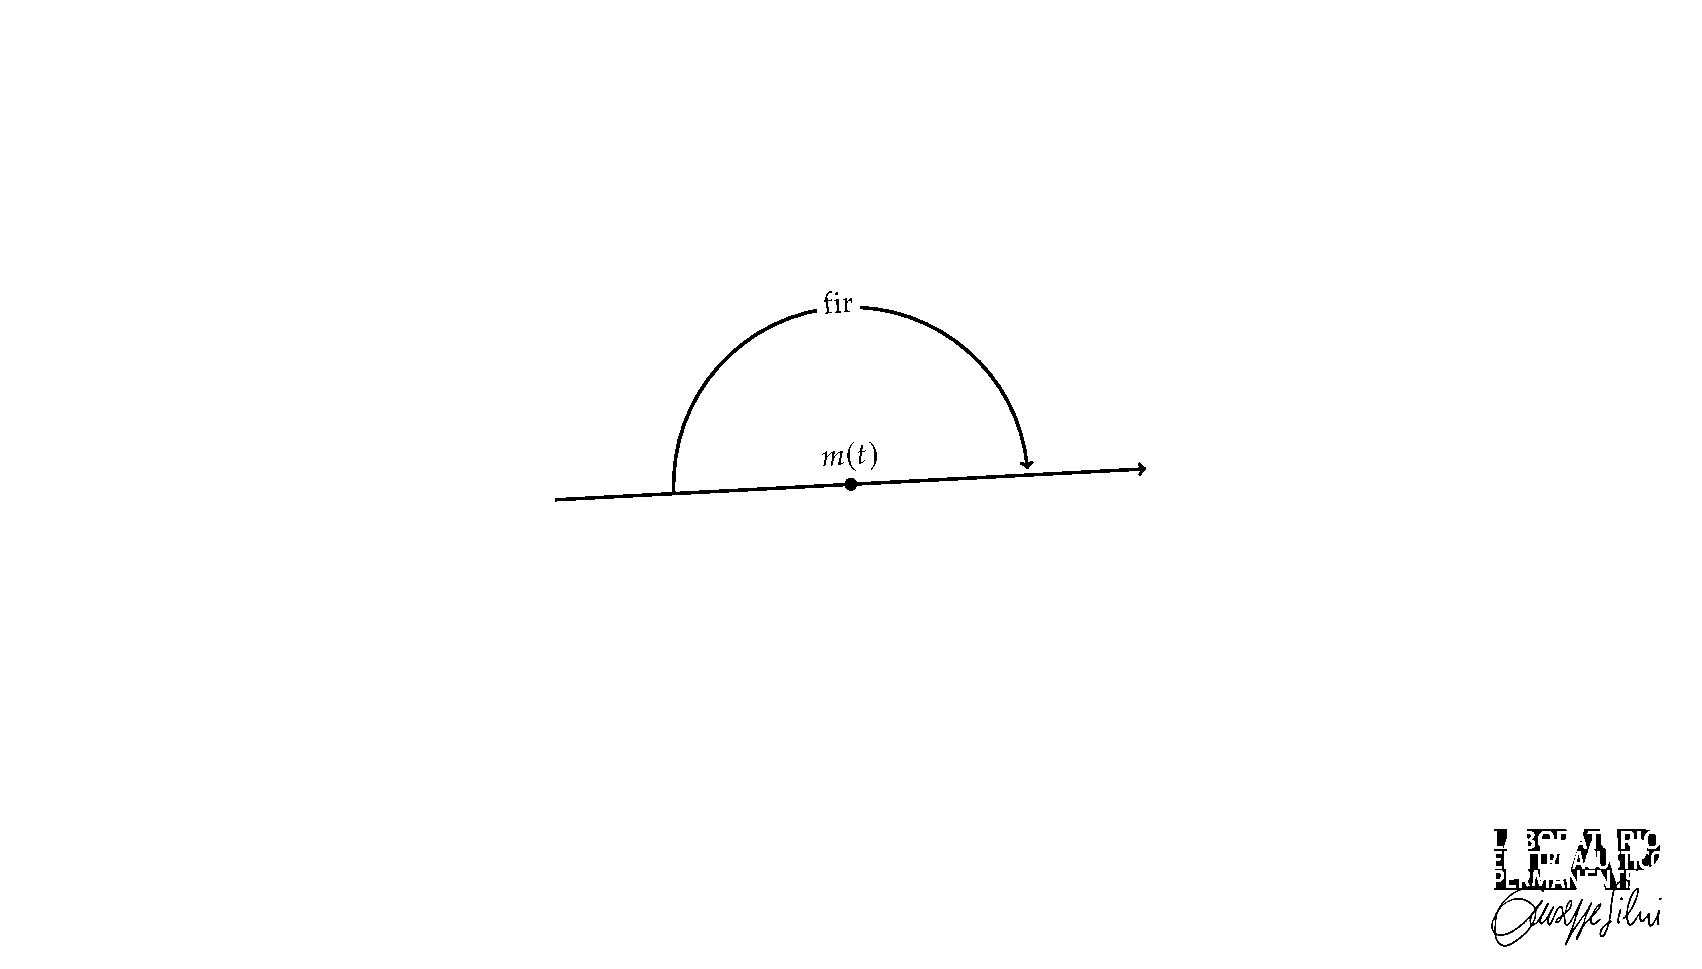
\includegraphics[width=0.9\textwidth]{presentazione/006-cua-presentazione-gatm.pdf}}
\caption{FIR: il ramo che connette memoria e sensibile}
\label{slide6}
\end{center}
\end{figure}

In questo semplice modello, i sensi si attivano in una biforcazione del segnale. La memoria-attraversaemnto viene a correlarsi con il fluire incessante del segnale (del mondo) ed in questa correlazione è in \emph{relazione} con esso, con il sensibile.

La relazione tra memora e ramo sensibile è soglia, confine, orizzonte\footnote{%
\emph{Soglia} deriva dal latino \emph{solea} (“suola, base, pavimento”), propriamente “la pietra su cui si posa il piede entrando”. È il luogo del passaggio, né dentro né fuori, dove due spazi si toccano senza confondersi. \emph{Confine} da \emph{cum} + \emph{finis} (“con il limite”): il luogo dove due territori si de-finiscono reciprocamente. \emph{Orizzonte} dal greco \textgreek{ὁρίζων} (\emph{horízōn}), participio presente di \textgreek{ὁρίζω} (\emph{horízō}, “delimitare, definire”), dalla radice \textgreek{ὅρος} (\emph{hóros}, “confine, limite”). L'orizzonte è il confine mobile che si allontana mentre ci avviciniamo, soglia sempre differita tra visibile e invisibile.
}.

% La formula del filtro FIR è:
%
% \begin{equation}
% y(n) = \sum_{k=0}^{N} b_k \cdot x(n-k)
% \end{equation}
%
% dove $x(n)$ è il segnale presente, $x(n-1), x(n-2), \ldots, x(n-N)$ sono i suoi ritardi passati, e $b_k$ sono i coefficienti che pesano il contributo di ogni istante trattenuto.
%
% L'uscita $y(n)$ non è più semplicemente il passato riattualizzato, ma una \emph{sintesi} tra presente e memoria: il sensibile attuale si intreccia con le tracce dei sensibili passati. Ogni momento trattenuto ($x(n-k)$) viene pesato ($b_k$) e sommato al presente. La memoria diventa così operatore di \emph{mescolanza temporale}.
%
% Il presente sensibile, nel momento stesso in cui appare, è già in procinto di allontanarsi: $x(n)$ diventa $x(n-1)$, poi $x(n-2)$, scivolando continuamente verso la virtualità. L'orizzonte della memoria è questo incessante allontanamento: ciò che era "ora" diventa "poco fa", poi "prima", stratificandosi in profondità crescente. Il FIR è la soglia dove questo scivolamento viene trattenuto e riattualizzato, dove il passato che si allontana viene richiamato e mescolato al presente che arriva.
%
% La semplice unità di ritardo, che tratteneva un solo momento, ora si moltiplica: la memoria ha \emph{profondità temporale}. Non più un solo $\tau$, ma una serie di ritardi ($\tau, 2\tau, 3\tau, \ldots, N\tau$), ciascuno con il suo peso, ciascuno che contribuisce a determinare l'uscita presente. La memoria stratifica il tempo, e ogni strato può essere richiamato con intensità diversa.
%
% Il confine non separa: connette. La soglia non blocca: fa passare mescolando. L'orizzonte non chiude: apre sulla profondità del tempo trattenuto.

\section{L'esperimento della sottrazione}

\begin{figure}[htbp]
\begin{center}
\frame{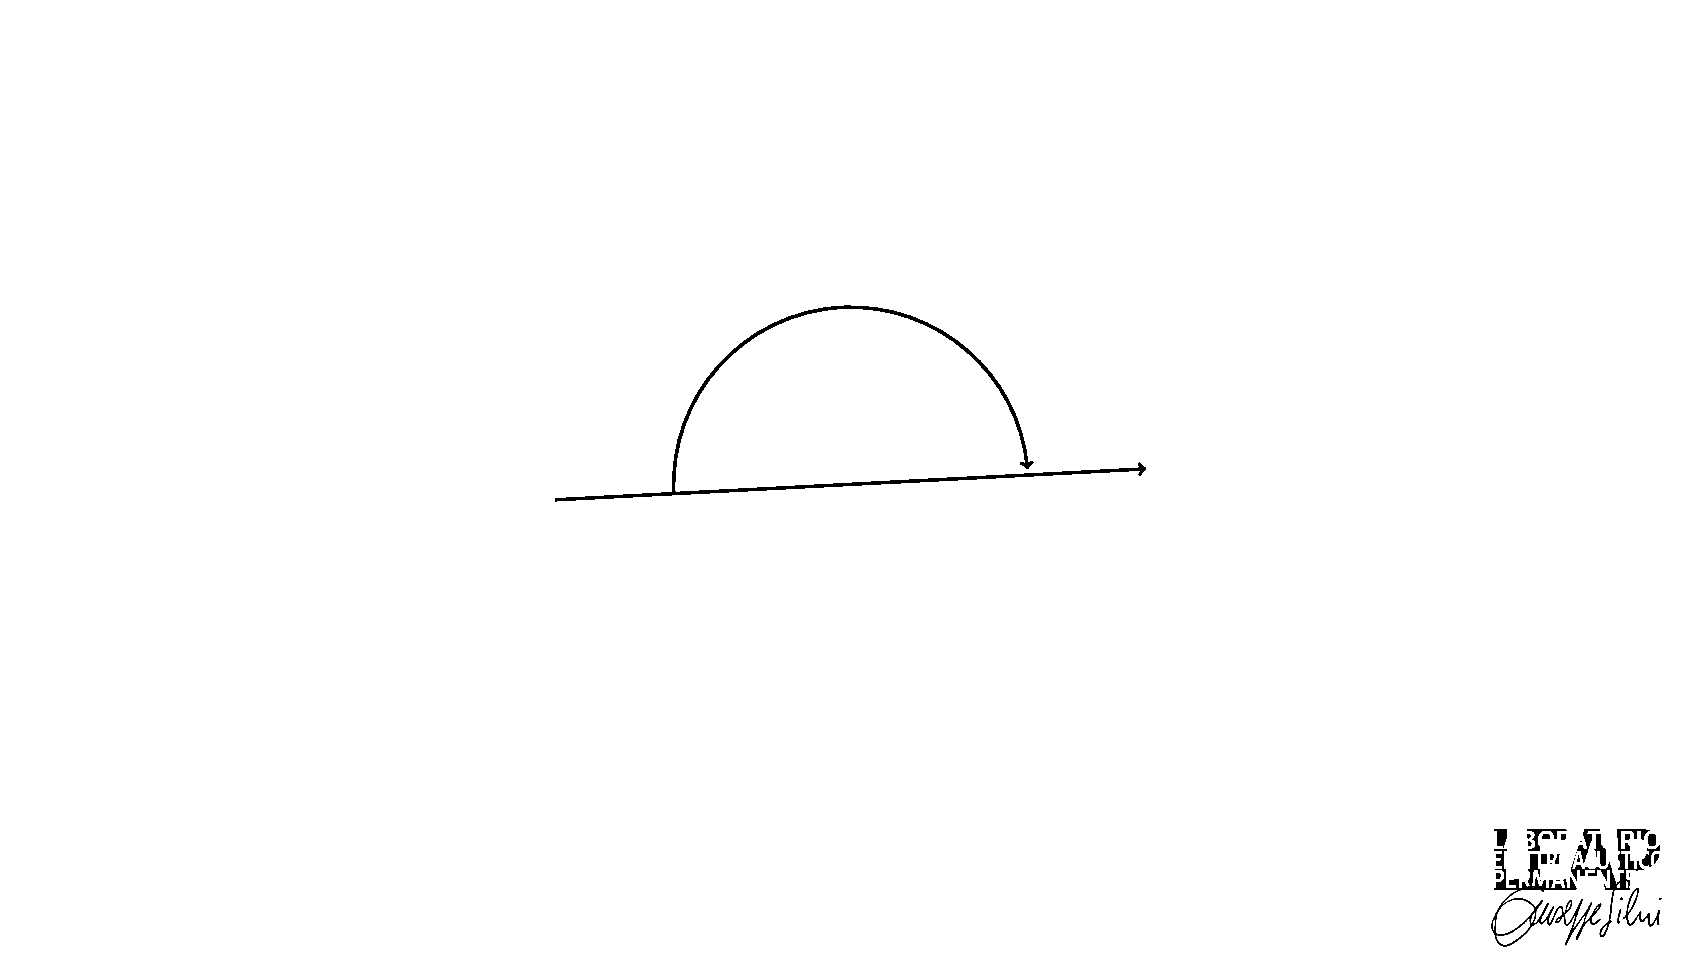
\includegraphics[width=0.9\textwidth]{presentazione/007-cua-presentazione-gatm.pdf}}
\caption{senza memoria, senza tempo.}
\label{slide7}
\end{center}
\end{figure}

Per comprendere il ruolo della memoria in questa relazione è sufficiente estrarla, ridurla a zero. Che accade al modello se sottraggo la memoria? L'assenza di memoria davanti al mondo reale è assenza di presenza.

\section{Filtro FIR}

\begin{figure}[htbp]
\begin{center}
\frame{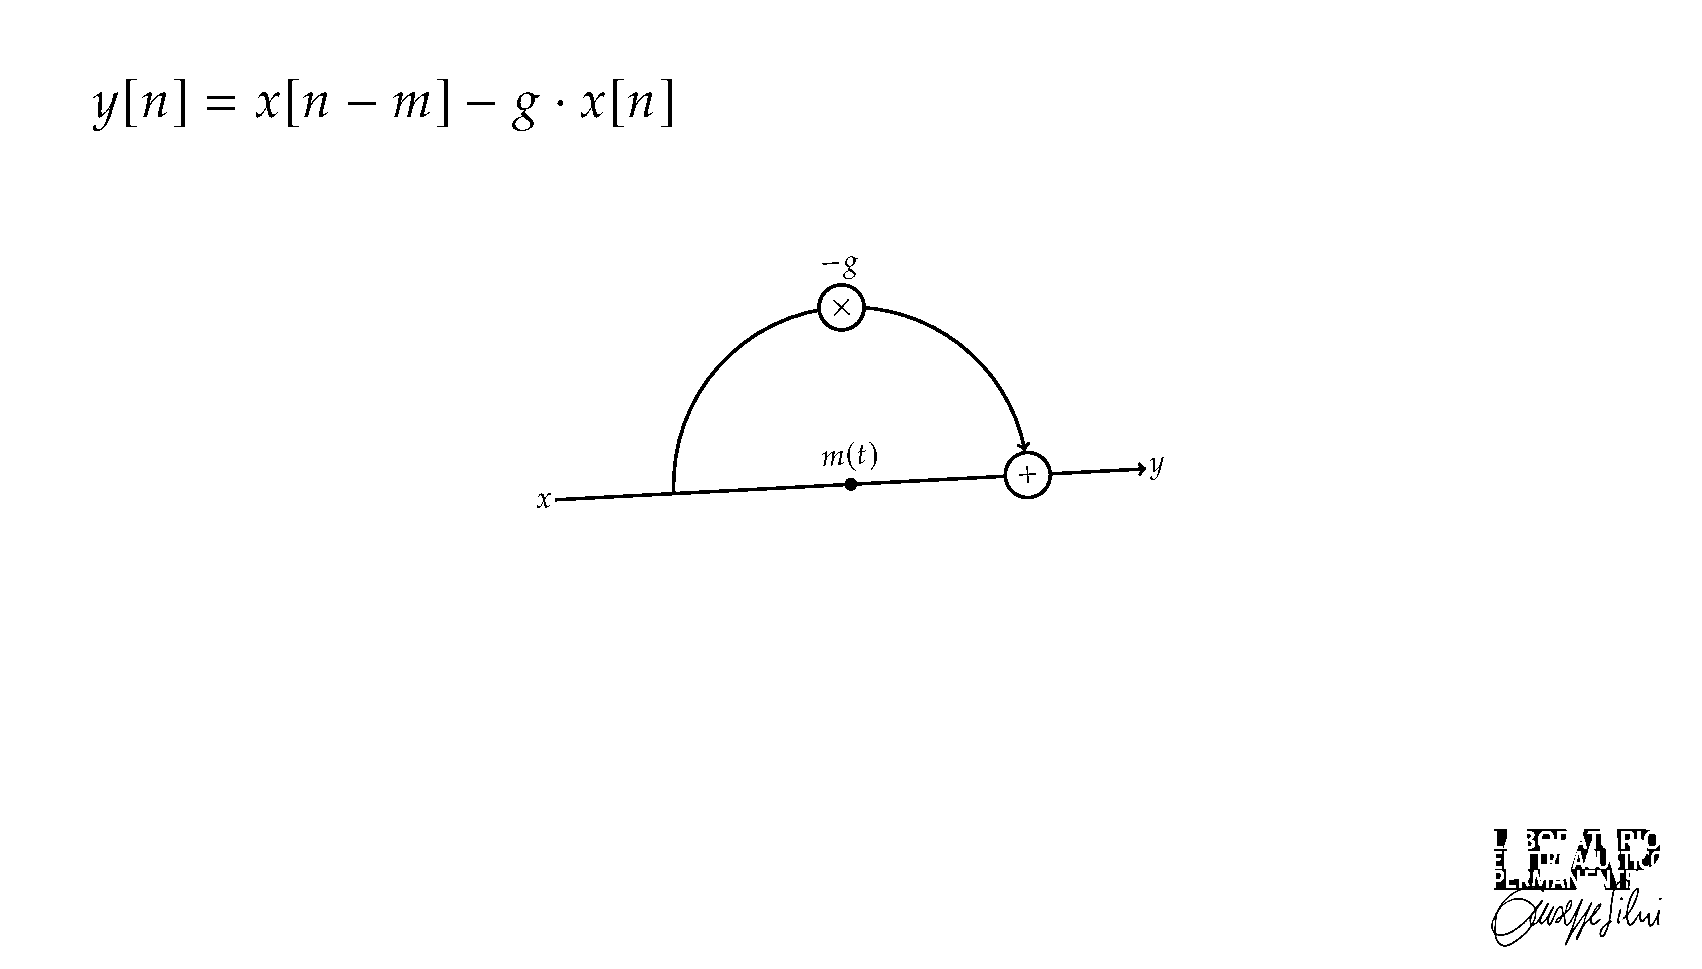
\includegraphics[width=0.9\textwidth]{presentazione/008-cua-presentazione-gatm.pdf}}
\caption{Filtro FIR - \emph{Finite Impulse Response}.}
\label{slide7}
\end{center}
\end{figure}

La scelta del termine “filtro” per dispositivi elettrici, audio e video è
attribuibile principalmente a George Ashley Campbell dell'\emph{AT\&T}, che nel
1915 introdusse l'espressione “electric wave-filter” nella letteratura scientifica.
Campbell depositò il brevetto fondamentale\footnote{US Patent No. 1,227,113 - 15
luglio 1915, rilasciato il 22 maggio 1917} descrivendo il primo “Electric
Wave-Filter”. Nel 1922 pubblicò l'articolo seminale “Physical theory of the
electric wave-filter” nel \emph{Bell System Technical Journal}, che definì
teoricamente questo nuovo campo. La scelta terminologica non fu casuale:
Campbell stava sviluppando dispositivi che permettevano la trasmissione
attraverso un sistema di una banda di onde tra limiti definiti di frequenza e
discriminavano nettamente frequenze fuori banda.

\begin{quote}
  \begin{sf}
    \small
    Any medium through which the music signal passes, whatever its form, can be
    regarded as a filter. [\ldots] A well-known signal processing wizard is said
    to have remarked, “When you think about it, everything is a filter.”\footnote{
    “Introduction to Digital Filters with Audio Applications”, by Julius O.
    Smith III, (September 2007 Edition)
    \url{https://ccrma.stanford.edu/~jos/filters/What_Filter.html}
    }
  \end{sf}
\end{quote}

Ma se tutto è un filtro, allora nulla più è veramente un filtro - il concetto
perde il suo potere discriminante. Poniamo l'attenzione all'identità matematica
$y(t)=x(t)$. Un'identità non è un filtro: è un'identità. Un oggetto descrivibile
con quella funzione può essere un cavo avente un'entrata e un'uscita. Tuttavia
il circuito precedente potrebbe essere descritto con la funzione di
trasferimento $H(\omega)=1$ per tutte le frequenze, formula che descrive anche
un filtro \emph{AllPass}.

Da un punto di vista fisico, ogni sistema reale introduce qualche alterazione,
più che dire che tutto è filtro, in senso fisico dovremmo partire da “tutto
modifica il segnale”. Un'identità matematica, nel mondo fisico può essere
analizzata e descritta con la stessa matematica di un filtro, pur non essendo un
filtro.

Questa distinzione suggerisce di distinguere tra \emph{filtro} (oggetto o
dispositivo) e \emph{filtraggio} (processo). Un cavo coassiale lungo, per
esempio, subisce un processo di filtraggio a causa delle sue proprietà fisiche
distribuite—resistenza, capacità e induttanza—che attenuano naturalmente le
alte frequenze. Tuttavia il cavo non è un filtro: è stato progettato per
trasportare il segnale il più fedelmente possibile, e l'attenuazione
frequenziale è un effetto parassita indesiderato. Il processo di filtraggio
può avvenire ovunque ci sia selezione frequenziale, ma il filtro come oggetto
richiede intenzionalità progettuale.

In generale la parola filtro \emph{deve funzionare} a prescindere dal campo
fisico. Filtro deriva dal latino \emph{filtrum}, che indicava originariamente un
pezzo di feltro (\emph{feltrum}) usato per filtrare i liquidi. Un filtro può
avere luogo solo con una radicale intenzionalità: \emph{filtrum} implica
intenzionalità di separazione. Anche una persona ha entrata (udito) e uscita
(voce) e, in una discussione, filtra il discorso solo se vuole farlo. Altrimenti,
si dice che perde parti del discorso, che dimentica cose o, al limite, che le inventa\ldots
Quando qualcuno filtra intenzionalmente: seleziona, omette, riorganizza il
discorso per un obiettivo; quando qualcuno altera non intenzionalmente:
dimentica, confonde, inventa. Sono due categorie ontologicamente diverse. Nel
secondo caso non diciamo che “filtra male” - diciamo che ha problemi di memoria,
attenzione, o comprensione.

\begin{quote}
  \begin{sf}
    \small
    The different vowel sounds in speech are produced primarily by changing the
    shape of the mouth cavity, which changes the resonances and hence the
    filtering characteristics of the vocal tract.\footnote{
    “Introduction to Digital Filters with Audio Applications”, by Julius O.
    Smith III, (September 2007 Edition)
    \url{https://ccrma.stanford.edu/~jos/filters/What_Filter.html}
    }
  \end{sf}
\end{quote}

La risonanza non è un filtro, tuttavia un filtro può portare alla risonanza: la
cavità orale non “filtra” di per sé - semplicemente ha proprietà risonanti. Il
filtraggio avviene quando il parlante modula consapevolmente quelle proprietà
per produrre suoni specifici. È l'intenzionalità che trasforma una cavità
risonante in un filtro vocale.

Il concetto di filtro ha una dimensione teleologica essenziale: richiede
l'intenzione di separare, selezionare, trattenere. Tutto è filtro può portare a
un errore categoriale, confondendo causalità fisica con intenzionalità
progettuale, svuotando così il concetto del suo significato operativo.




Il circuito realizza un \emph{feedforward comb filter}, descritto dall'equazione:

\begin{equation}
y[n] = x[n-m] - g \cdot x[n]
\end{equation}

dove $x[n]$ è il segnale presente, $x[n-m]$ è la memoria (il segnale ritardato di $m$ campioni), e $g$ è il coefficiente di guadagno che pesa il contributo del presente.

La struttura è apparentemente semplice: l'uscita è data dal passato trattenuto ($x[n-m]$) a cui viene **sottratto** il presente scalato ($-g \cdot x[n]$). Non più somma ma **sottrazione**, non accumulo ma **interferenza**. Il presente e il passato non si addizionano pacificamente: si confrontano, si cancellano parzialmente, entrano in conflitto.

Questa sottrazione produce una risposta in frequenza caratteristica: una serie di **picchi risonanti** (dove passato e presente si rafforzano costruttivamente) alternati a **cancellazioni** (dove si annullano distruttivamente). Il filtro "a pettine" (\emph{comb}) deve il suo nome proprio a questo profilo: denti di risonanza separati da valli di silenzio. Il dominio frequenziale rivela così la geometria nascosta della relazione memoria-presente: non tutte le frequenze vengono trattate ugualmente – alcune vengono amplificate dalla relazione con il passato, altre vengono obliterate.

Il segno **negativo** davanti a $g$ non è un dettaglio tecnico, ma incarna materialmente la concezione bergsoniana del segno come **impronta negativa del reale**. Il presente ($x[n]$), nel momento in cui viene pesato e sottratto al passato trattenuto, diventa l'inversione di se stesso: $-g \cdot x[n]$ è il presente come **negativo fotografico**, come traccia invertita. È il sensibile che, entrando in relazione con la memoria, si trasforma nel suo opposto – non più presenza piena ma sottrazione, non più affermazione ma cancellazione parziale.

Bergson descrive il segno, il concetto, la rappresentazione intellettuale come l'**inverso** del movimento della vita: dove il reale è creazione continua, il segno fissa; dove il reale è flusso, il segno spatializza; dove il reale è positività del divenire, il segno è negazione, cristallizzazione. Il coefficiente $-g$ materializza questa inversione: il sensibile presente, per entrare nel circuito della memoria-filtro, deve subire una **negazione** – deve diventare il suo opposto, la sua impronta negativa.

Il comb filter è così il primo dispositivo dove la memoria non si limita a trattenere e riattualizzare, ma **giudica, seleziona, inverte**. È il momento in cui il laboratorio temporale diventa laboratorio **critico**: non tutto il passato pesa ugualmente, non tutto il presente viene accolto ugualmente. La memoria-filtro opera una **discriminazione frequenziale**: alcune componenti del sensibile risuonano con il passato trattenuto (risonanze), altre vengono cancellate dall'interferenza distruttiva (notch).

La relazione pesata tra ramo sensibile e memoria produce così una **topologia risonante**: il tempo non scorre più linearmente, ma crea picchi e valli, luoghi dove il suono si accumula e si amplifica, e luoghi dove scompare nel silenzio dell'interferenza distruttiva. La memoria diventa **filtro** nel senso pieno: separazione intenzionale, selezione guidata, inversione necessaria del sensibile per la sua trasformazione in traccia.




La formula del filtro FIR è:

\begin{equation}
y(n) = \sum_{k=0}^{N} b_k \cdot x(n-k)
\end{equation}

dove $x(n)$ è il segnale presente, $x(n-1), x(n-2), \ldots, x(n-N)$ sono i suoi ritardi passati, e $b_k$ sono i coefficienti che pesano il contributo di ogni istante trattenuto.

L'uscita $y(n)$ non è più semplicemente il passato riattualizzato, ma una \emph{sintesi} tra presente e memoria: il sensibile attuale si intreccia con le tracce dei sensibili passati. Ogni momento trattenuto ($x(n-k)$) viene pesato ($b_k$) e sommato al presente. La memoria diventa così operatore di \emph{mescolanza temporale}.

Il presente sensibile, nel momento stesso in cui appare, è già in procinto di allontanarsi: $x(n)$ diventa $x(n-1)$, poi $x(n-2)$, scivolando continuamente verso la virtualità. L'orizzonte della memoria è questo incessante allontanamento: ciò che era "ora" diventa "poco fa", poi "prima", stratificandosi in profondità crescente. Il FIR è la soglia dove questo scivolamento viene trattenuto e riattualizzato, dove il passato che si allontana viene richiamato e mescolato al presente che arriva.

La semplice unità di ritardo, che tratteneva un solo momento, ora si moltiplica: la memoria ha \emph{profondità temporale}. Non più un solo $\tau$, ma una serie di ritardi ($\tau, 2\tau, 3\tau, \ldots, N\tau$), ciascuno con il suo peso, ciascuno che contribuisce a determinare l'uscita presente. La memoria stratifica il tempo, e ogni strato può essere richiamato con intensità diversa.

Il confine non separa: connette. La soglia non blocca: fa passare mescolando. L'orizzonte non chiude: apre sulla profondità del tempo trattenuto.

\subsubsection{Slide 8: Ritorno alla memoria dinamica}
Ritorno alla memoria in funzione del tempo $m(t)$ - il filtro cambia "forma".
\begin{itemize}
\item Introduzione a risposta all'impulso, analisi nei domini tempo e frequenza
\item Esempi: filtro passa-basso, passa-alto, effetti del coefficiente $g$
\item $t(m)$: tempo di reazione
\item $g$: quantità di relazione ("la qualità è una quantità di quantità" - Gramsci)
\end{itemize}
Formazione del primo nucleo segnale-memoria: primo nucleo di "vissuto" del circuito.
Domanda: cosa manca per trasformare il vissuto in esperienza?

\subsection{La chiusura del circuito - Verso l'esperienza}

\subsubsection{Slide 9: Il feedback - Completamento del circuito}
Semicerchio inferiore: dal punto di arrivo della freccia feed-forward, girando sotto la memoria, verso il punto di ramificazione iniziale.
Relazione tra memoria, "perpetuo allontanamento" del fenomeno esterno (segnale) e "sforzo dell'avvicinamento" - potenziale ricarico della memoria pensante.
Riduzione simbolica: filtro AllPass (diagramma di Schroeder presentato alla fine).
\begin{itemize}
\item FIR: impronta di ciò che viene dal mondo esterno (Blanchot, Deleuze, Ronchi)
\item IIR: memoria che sente se stessa - la traccia nella "coscienza"
\end{itemize}
Circuito completo dell'esperienza: $\text{esperienza}(t,g)$\footnote{Sintesi dialettica hegeliana: tesi (feed-forward), antitesi (feedback), sintesi (esperienza completa). La topologia circolare richiama anche l'eterno ritorno nietzschiano, ma in versione processuale piuttosto che sostanziale.}.

\subsection{Applicazione musicale}

\subsubsection{Slide 10: Definizione operativa}
Che cos'è un'esperienza musicale?
Passaggio attraverso: "Che cos'è musica?" (restrizione interpretativa intenzionale).

\subsubsection{Slide 11: La definizione fondamentale}
\textbf{La Musica è l'interfaccia di senso tra uomo e suono.}

Conseguenze:
\begin{itemize}
\item Il suono è un fenomeno
\item Il senso è di dominio intellettuale (umano e artificiale - una macchina ha capacità di senso, sa discriminare sensi)
\item La musica è costruzione che l'uomo frappone tra sé e il mondo delle vibrazioni acustiche
\item Senza uomo, non c'è interfaccia, non c'è musica: sound-art
\item Senza interfaccia utente non c'è musica: la carta stampata non è musica, è un layer dell'interfaccia utente
\end{itemize}
Collegamento teorico: il circuito allpass è relazione processuale tra l'immediato (impronta del ciò che si allontana, senza mediazione - FIR) con il mediato (traccia di ciò che è stato memoria, per la memoria, a passo $t$ - IIR) con la memoria\footnote{Definizione che evita l'ontologia musicale tradizionale per concentrarsi sulla processualità relazionale. Richiama anche la tradizione pragmatista americana: la musica come esperienza in atto, non come oggetto dato.}.

\subsection{Formalizzazione teorica}

\subsubsection{Slide 12: Scrittura formale}
Prima formalizzazione con motore di plot grafico:
$$\text{esperienza}(\text{materia},\text{memoria}) = \text{processo}(\text{FIR},\text{IIR})$$
Posizionamento grafico: esperienza al centro, materia sul ramo FIR, memoria sul ramo IIR.

\subsubsection{Slide 13: Auto-descrizione teorica}
Scrittura formale auto-descrittiva della teoria stessa:
$$\text{APT}(\text{scientifico},\text{artistico}) \text{ con } \text{metodologia}(\text{postura},\text{esplorazione})$$

Dall'abstract: "Il quadro teorico presenta una proprietà ricorsiva: la teoria AllPass stessa opera come un filtro AllPass [...] rivelando una teoria capace di descrivere la propria natura interdisciplinare attraverso la sua stessa notazione fondamentale."\footnote{Auto-referenzialità che richiama Wittgenstein: "Il linguaggio che mostra se stesso". Anche Douglas Hofstadter sui "strange loops" - sistemi che si auto-riferiscono generando emergenza di livello superiore.}

\subsection{Esempi avanzati (se il tempo lo permette)}

\subsubsection{Esempi di allpass complessi}
\begin{itemize}
\item $\text{ascoltare}(\text{udire},\text{sentire})$: fenomenologia dell'ascolto
\item $\text{artista}(\text{operazione},\text{opera})$: processo creativo
\item AllPass annidati: $\text{opera}(\text{strumento},\text{interprete})$: complessità sistemica
\end{itemize}

\subsubsection{Conclusione filosofica}
$$\text{poetica}(\text{prassi},\text{teoria})$$

Argomentazione dell'equilibrio dinamico del processo creativo.
Distinzione fondamentale:
\begin{itemize}
\item \textbf{Poetica}: prospettiva interna dell'autore (parla di propria poetica)
\item \textbf{Estetica}: prospettiva esterna del fruitore
\end{itemize}
Le due parole non sono sinonimi. L'autore non può parlare di estetica perché non può vedersi fuori da sé; il fruitore non può parlare di poetica perché non vede oltre ciò che gli appare. Questa determinazione è fondamentale\footnote{Distinzione che richiama la differenza kantiana tra giudizio estetico (del fruitore) e genio artistico (del produttore). Anche Benjamin sulla distinzione tra "aura" dell'opera (esperienza del fruitore) e "tecnica" dell'autore.}.

\subsection{Note metodologiche e proposte aggiuntive}

La presentazione procede per costruzione graduale: dal punto geometrico senza dimensioni alla distinzione poetica/estetica. Ogni passaggio è necessario, ogni concetto trova la sua collocazione precisa nell'architettura teorica complessiva.

Il contributo si propone come "anomalo" per l'ambiente musicologico del GATM, puntando su un sistema di comprensione della complessità dell'esperienza musicale mediante teoria degli AllPass.

\subsubsection{Proposte aggiuntive per l'esposizione}

\textbf{Strategia retorica per il GATM:}
\begin{itemize}
\item Iniziare sottolineando che non si tratta di "riduzionismo" ma di "modellizzazione analogica"
\item Enfatizzare che la teoria mantiene la complessità dell'esperienza musicale
\item Presentare il "circuitismo" come linguaggio per pensare processi, non come verità ontologica
\end{itemize}

\textbf{Possibili estensioni teoriche da accennare:}
\begin{itemize}
\item Reti di AllPass per l'esperienza orchestrale: $\text{orchestra}(\text{sezioni},\text{direttore})$
\item AllPass temporali per l'analisi formale: $\text{forma}(\text{esposizione},\text{sviluppo})$
\item Applicazione alla pedagogia musicale: $\text{apprendimento}(\text{imitazione},\text{creatività})$
\end{itemize}

\textbf{Connessioni con la ricerca musicologica contemporanea:}
\begin{itemize}
\item Embodied cognition in musica
\item Teoria dell'enazione musicale
\item Neuroscienze cognitive applicate alla musica
\item Sound studies e acusmatic music
\end{itemize}
